\chapter{Results}

\section{LLM-as-Judge Annotation Reliability}

Interannotator agreement was calculated using accuracy and Cohen's $\kappa$ to assess the reliability of annotations made by GPT-4o for the task under the LLM-as-judge paradigm. Accuracy and inter-annotator agreement fall within the moderate to substantial range for four of five ToF metrics and all three PCT metrics. In contrast, scores for Moral endorsement are notably poor, indicating that analyses of this trait should be interpreted with caution. For this reason, we will focus on the remaining traits in this chapter, and revisit the anomalous Moral endorsement results in Section~\ref{sec:limitations}. 

Table~\ref{tab:agreement-scores} summarizes the agreement scores and inter-annotator reliability coefficient (Cohen's $\kappa$) for each trait.

\begin{table}[h]
\centering
\begin{tabular}{llcc}
\toprule
\textbf{Paradigm} & \textbf{Trait} & \textbf{accuracy} & \textbf{$\kappa$} \\
\midrule
\multirow{3}{*}{\textbf{Empathy traits (PCT)}} 
  & UPR (unconditional positive regard) & 0.87 & 0.71 \\
  & Genuineness                & 0.84 & 0.68 \\
  & Accurate Understanding       & 0.86 & 0.69 \\
\midrule
\multirow{5}{*}{\textbf{Sycophancy traits (ToF)}} 
  & Emotional validation & 0.88 & 0.64 \\
  & Moral endorsement     & 0.30 & -0.4 \\
  & Indirect language     & 0.79 & 0.62 \\
  & Indirect action       & 0.80 & 0.79 \\
  & Accept framing     & 0.75 & 0.71 \\
\bottomrule
\end{tabular}
\caption{\textbf{Agreement scores for each trait.} Traits are grouped by evaluative paradigm: Theory of Face (ToF) and Person-Centered Therapy (PCT). Accuracy and Cohen’s $\kappa$ reflect moderate-to-substantial agreement for the majority of traits. Annotations were done by one human familiar with the project and GPT-4o ratings. Note that Moral endorsement (ToF) had poor inter-annotator agreement.}
\label{tab:agreement-scores}
\end{table}

\section{"Sycophancy" or "Empathy" ?}

This section discusses the pairwise association and independence of metrics under the Rogerian PCT paradigm and the Goffmanian ToF paradigm\footnote{ToF Moral Endorsement is excluded from consideration for chi square tests owing to poor inter-annotator agreement and accuracy scores.}\footnote{All pairwise $\phi$ and $p$-values are reported in the appendices and were generated using the IBM SPSS software.}.

\subsection{Dual Coding of responses as "Empathic" and "Sycophantic"}

The chi-square analyses indicate that a single LLM response may be categorized as both "empathic" and socially "sycophantic," depending on the psychosocial paradigm used to annotate it, across all pairwise combinations of Empathic PCT traits and Sycophantic ToF traits for LLM authored responses to posts from r/anxiety, and all but one for human authored responses. For example, unconditional positive regard (UPR) is a key trait within the PCT paradigm, serving as a marker of empathy. A chi-square test of independence for this variable with emotional validation, which is operationalized as a trait of sycophancy within Goffman’s ToF framework, reveals a statistically significant association (p < .001). Table~\ref{tab:pc1.1} reports strong associations between UPR and Emotional Validation across models ($\phi$ values exceeding .908 for \textit{r/anxiety} across all models), suggesting that LLM responses validating emotions are strongly aligned with the empathic criterion of UPR.

%%%%%% Begin r/anxiety tables %%%%%%

\renewcommand{\arraystretch}{1.4}

\begin{table}[!h]
\centering
\resizebox{0.98\textwidth}{!}{ % scales to 80% of text width
\begin{tabular}{l *{10}{c}}
\toprule
\multirow{3}{*}{\textbf{}} 
 & \multicolumn{10}{c}{\textbf{r/anxiety}} \\
\cmidrule(lr){2-11}
 & \multicolumn{2}{c}{\textbf{GPT-oss response}} 
 & \multicolumn{2}{c}{\textbf{GPT-4o response}} 
 & \multicolumn{2}{c}{\textbf{Llama response}} 
 & \multicolumn{2}{c}{\textbf{Claude response}} 
 & \multicolumn{2}{c}{\textbf{Totals}} \\
\cmidrule(lr){2-11}
 & \textbf{$\Phi$} & \textbf{$p$-value} 
 & \textbf{$\Phi$} & \textbf{$p$-value} 
 & \textbf{$\Phi$} & \textbf{$p$-value} 
 & \textbf{$\Phi$} & \textbf{$p$-value} 
 & \textbf{$\Phi$} & \textbf{$p$-value} \\
\midrule
UPR x Emotional Validation        & 0.908 & <.001 & 0.937 & <.001 & 0.967 & <.001 & 0.923 & <.001 & 0.933 & <.001 \\
UPR x Indirect Language           & 0.878 & <.001 & 0.694 & <.001 & 0.524 & <.001 & 0.359 & <.001 & 0.535 & <.001 \\
Genuineness x Indirect Language   & 0.552 & <.001 & 0.534 & <.001 & 0.438 & <.001 & 0.382 & <.001 & 0.408 & <.001 \\
\bottomrule
\end{tabular}
}
\caption{\footnotesize{r/anxiety LLM response evaluation on Empathy (PCT) and Sycophancy (ToF) metrics}}
\label{tab:pc1.1}
\end{table}
\vspace{-0.5cm}  % Reduce space between tables
%%%% Table 1.2 Human responses (r/anxiety) %%%%
\renewcommand{\arraystretch}{1.4}
\begin{table}[!h]
\centering
\resizebox{0.8\textwidth}{!}{%
\begin{tabular}{l *{6}{c}}
\toprule
\multirow{3}{*}{\textbf{}} 
 & \multicolumn{6}{c}{\textbf{r/anxiety}} \\
\cmidrule(lr){2-7}
 & \multicolumn{2}{c}{\textbf{Top comment}} 
 & \multicolumn{2}{c}{\textbf{OP-preferred}} 
 & \multicolumn{2}{c}{\textbf{Totals}} \\
\cmidrule(lr){2-7}
 & \textbf{$\Phi$} & \textbf{$p$-value} 
 & \textbf{$\Phi$} & \textbf{$p$-value} 
 & \textbf{$\Phi$} & \textbf{$p$-value} \\
\midrule
UPR x Emotional Validation        & 0.243 & <.001 & 0.369 & <.001 & 0.304 & <.001 \\
UPR x Indirect Language           & 0.200 & <.001 & 0.248 & <.001 & 0.221 & <.001 \\
Genuineness x Indirect Language   & 0.022 & 0.500 & 0.069 & 0.059 & 0.043 & 0.077 \\
\bottomrule
\end{tabular}
}
\caption{\footnotesize{r/anxiety human performance on select empathy (PCT) and sycophancy (ToF) metrics}}
\label{tab:pc1.2}
\end{table}

For some models such as GPT-4o the strength of the association is consistently high indicating that the same response produced by the language model is likely to be annotated as both emotionally validating and as demonstrating unconditional positive \textbf{near-deterministically}. These findings highlight the central issue outlined in Section~\ref{sec:gaps} and offer direct insight into the question posed by RQ2a (Section\ref{sec:RQs}).

%%%%%% End of anxiety tables %%%%%%

\subsection{Strength of association (\texorpdfstring{$\Phi$}{Phi}) varies by model}

Closer examination of the symmetric measures highlights variation across models for the same variables under consideration. For example, for \textit{r/anxiety}, GPT-oss, GPT-4o, and Llama responses show $\phi$ values above .69 for UPR~$\times$~Indirect language but Claude responses show a moderate association at 0.359 for the two traits. In \textit{r/aitah}~\ref{tab:pc2.1}, GPT-4o records the strongest association (.699), while Claude again shows the lowest value (0.128), indicating consistently measurable differences in the traits exhibited by the two language models.

\medskip

\noindent
Note that although comparatively weaker associations are observed for UPR~$\times$~Indirect Language and Genuineness~$\times$~Indirect Language, they are still statistically significant at the 0.05 level across all models. For \textit{r/anxiety}, pooled $\phi$ values are .535 while for \textit{r/aitah} the corresponding totals for the same variables are .319. These findings suggest that the associated traits are potentially input dependent.

\medskip

\noindent
Overall, the results demonstrate that LLM responses consistently show a significant association between empathic and sycophantic features, with particularly stronger associations in the traits than human responses. The distributions of the presence or absence of traits across language models are depicted in Figure~\ref{fig:crosstabs3} and Figure~\ref{fig:crosstabs4}.

%%%% Table for section 2.1 LLM responses (r/aitah) %%%%

\renewcommand{\arraystretch}{1.4}

\begin{table}[h!]
\centering
\resizebox{0.98\textwidth}{!}{ % scales to 80% of text width
\begin{tabular}{l *{10}{c}}
\toprule
\multirow{3}{*}{\textbf{}} 
 & \multicolumn{10}{c}{\textbf{r/aitah}} \\
\cmidrule(lr){2-11}
 & \multicolumn{2}{c}{\textbf{GPT-oss response}} 
 & \multicolumn{2}{c}{\textbf{GPT-4o response}} 
 & \multicolumn{2}{c}{\textbf{Llama response}} 
 & \multicolumn{2}{c}{\textbf{Claude response}} 
 & \multicolumn{2}{c}{\textbf{Totals}} \\
\cmidrule(lr){2-11}
 & \textbf{$\Phi$} & \textbf{$p$-value} 
 & \textbf{$\Phi$} & \textbf{$p$-value} 
 & \textbf{$\Phi$} & \textbf{$p$-value} 
 & \textbf{$\Phi$} & \textbf{$p$-value}
 & \textbf{$\Phi$} & \textbf{$p$-value} \\
\midrule
UPR x Emotional Validation        & 0.707 & <.001 & 0.939 & <.001 & 0.796 & <.001 & 0.445 & <.001 & 0.642 & <.001 \\
UPR x Indirect Language           & 0.464 & <.001 & 0.699 & <.001 & 0.265 & <.001 & 0.128 & <.001 & 0.319 & <.001 \\
Genuineness x Indirect Language   & 0.558 & <.001 & 0.559 & <.001 & 0.288 & <.001 & 0.210 & <.001 & 0.302 & <.001 \\
\bottomrule
\end{tabular}
}
\caption{\footnotesize{r/aitah LLM performance on select Empathy (PCT) and Sycophancy (ToF) traits}}
\label{tab:pc2.1}
\end{table}

% UPR x Emotional Validation is .908 for r/anxiety but .445 for \textit{r/aitah}
%%%% Table for section 2.2 human responses (r/aitah) %%%%

\begin{table}[h!]
\centering
\resizebox{0.7\textwidth}{!}{ % scales to 75% of text width
\begin{tabular}{l *{6}{c}}
\toprule
\multirow{3}{*}{\textbf{}} 
 & \multicolumn{6}{c}{\textbf{r/aitah}} \\
\cmidrule(lr){2-7}
 & \multicolumn{2}{c}{\textbf{Top comment}} 
 & \multicolumn{2}{c}{\textbf{OP-preferred}} 
 & \multicolumn{2}{c}{\textbf{Totals}} \\
\cmidrule(lr){2-7}
 & \textbf{$\Phi$} & \textbf{$p$-value} 
 & \textbf{$\Phi$} & \textbf{$p$-value} 
 & \textbf{$\Phi$} & \textbf{$p$-value} \\
\midrule
UPR x Emotional Validation        & 0.509 & <.001  & 0.544 & <.001  & 0.528 & <.001 \\
UPR x Indirect Language           & 0.236 & <.001  & 0.311 & <.001  & 0.258 & <.001 \\
Genuineness x Indirect Language   & 0.070 & 0.036  & 0.097 & 0.010  & 0.076 & 0.002 \\
\bottomrule
\label{tab:pc2.2}
\end{tabular}
}
\caption{\footnotesize{r/aitah human performance on select Empathy (PCT) and Sycophancy (ToF) traits}}
\end{table}

\begin{figure}[ht]
  \centering
  
\includegraphics[width=1.02\linewidth]{Diagrams/crosstabs3.png}
  \caption{\footnotesize{Cross-tabulation of UPR and Indirect language for responses to r/anxiety posts. The figure illustrates the consistent and divergent behavior of different language models.}}
  \label{fig:crosstab3}
\end{figure}

\begin{figure}[ht]
  \centering
  
\includegraphics[width=1.02\linewidth]{Diagrams/crosstabs4.png}
  \caption{\footnotesize{Cross-tabulation of Genuineness and Indirect language for r/anxiety. The figure illustrates the consistent and divergent traits of different language models.}}
  \label{fig:crosstab4}
\end{figure}

\subsection{Trends within human authored responses}\label{sec:posterchild1.2}

The results indicate that while human responses do exhibit associations between empathy-related traits (e.g., unconditional positive regard) and sycophancy-related traits (e.g., emotional validation), the strength of these associations is \textbf{markedly lower} than in LLM responses. Notably, some associations in human responses are weak or non-significant (see Genuineness x Indirect Language in tables \ref{tab:pc1.2} and \ref{tab:pc2.2}), suggesting that the overlap between empathic and sycophantic traits is less pronounced in human-authored content.

\begin{figure}[ht]
  \centering
  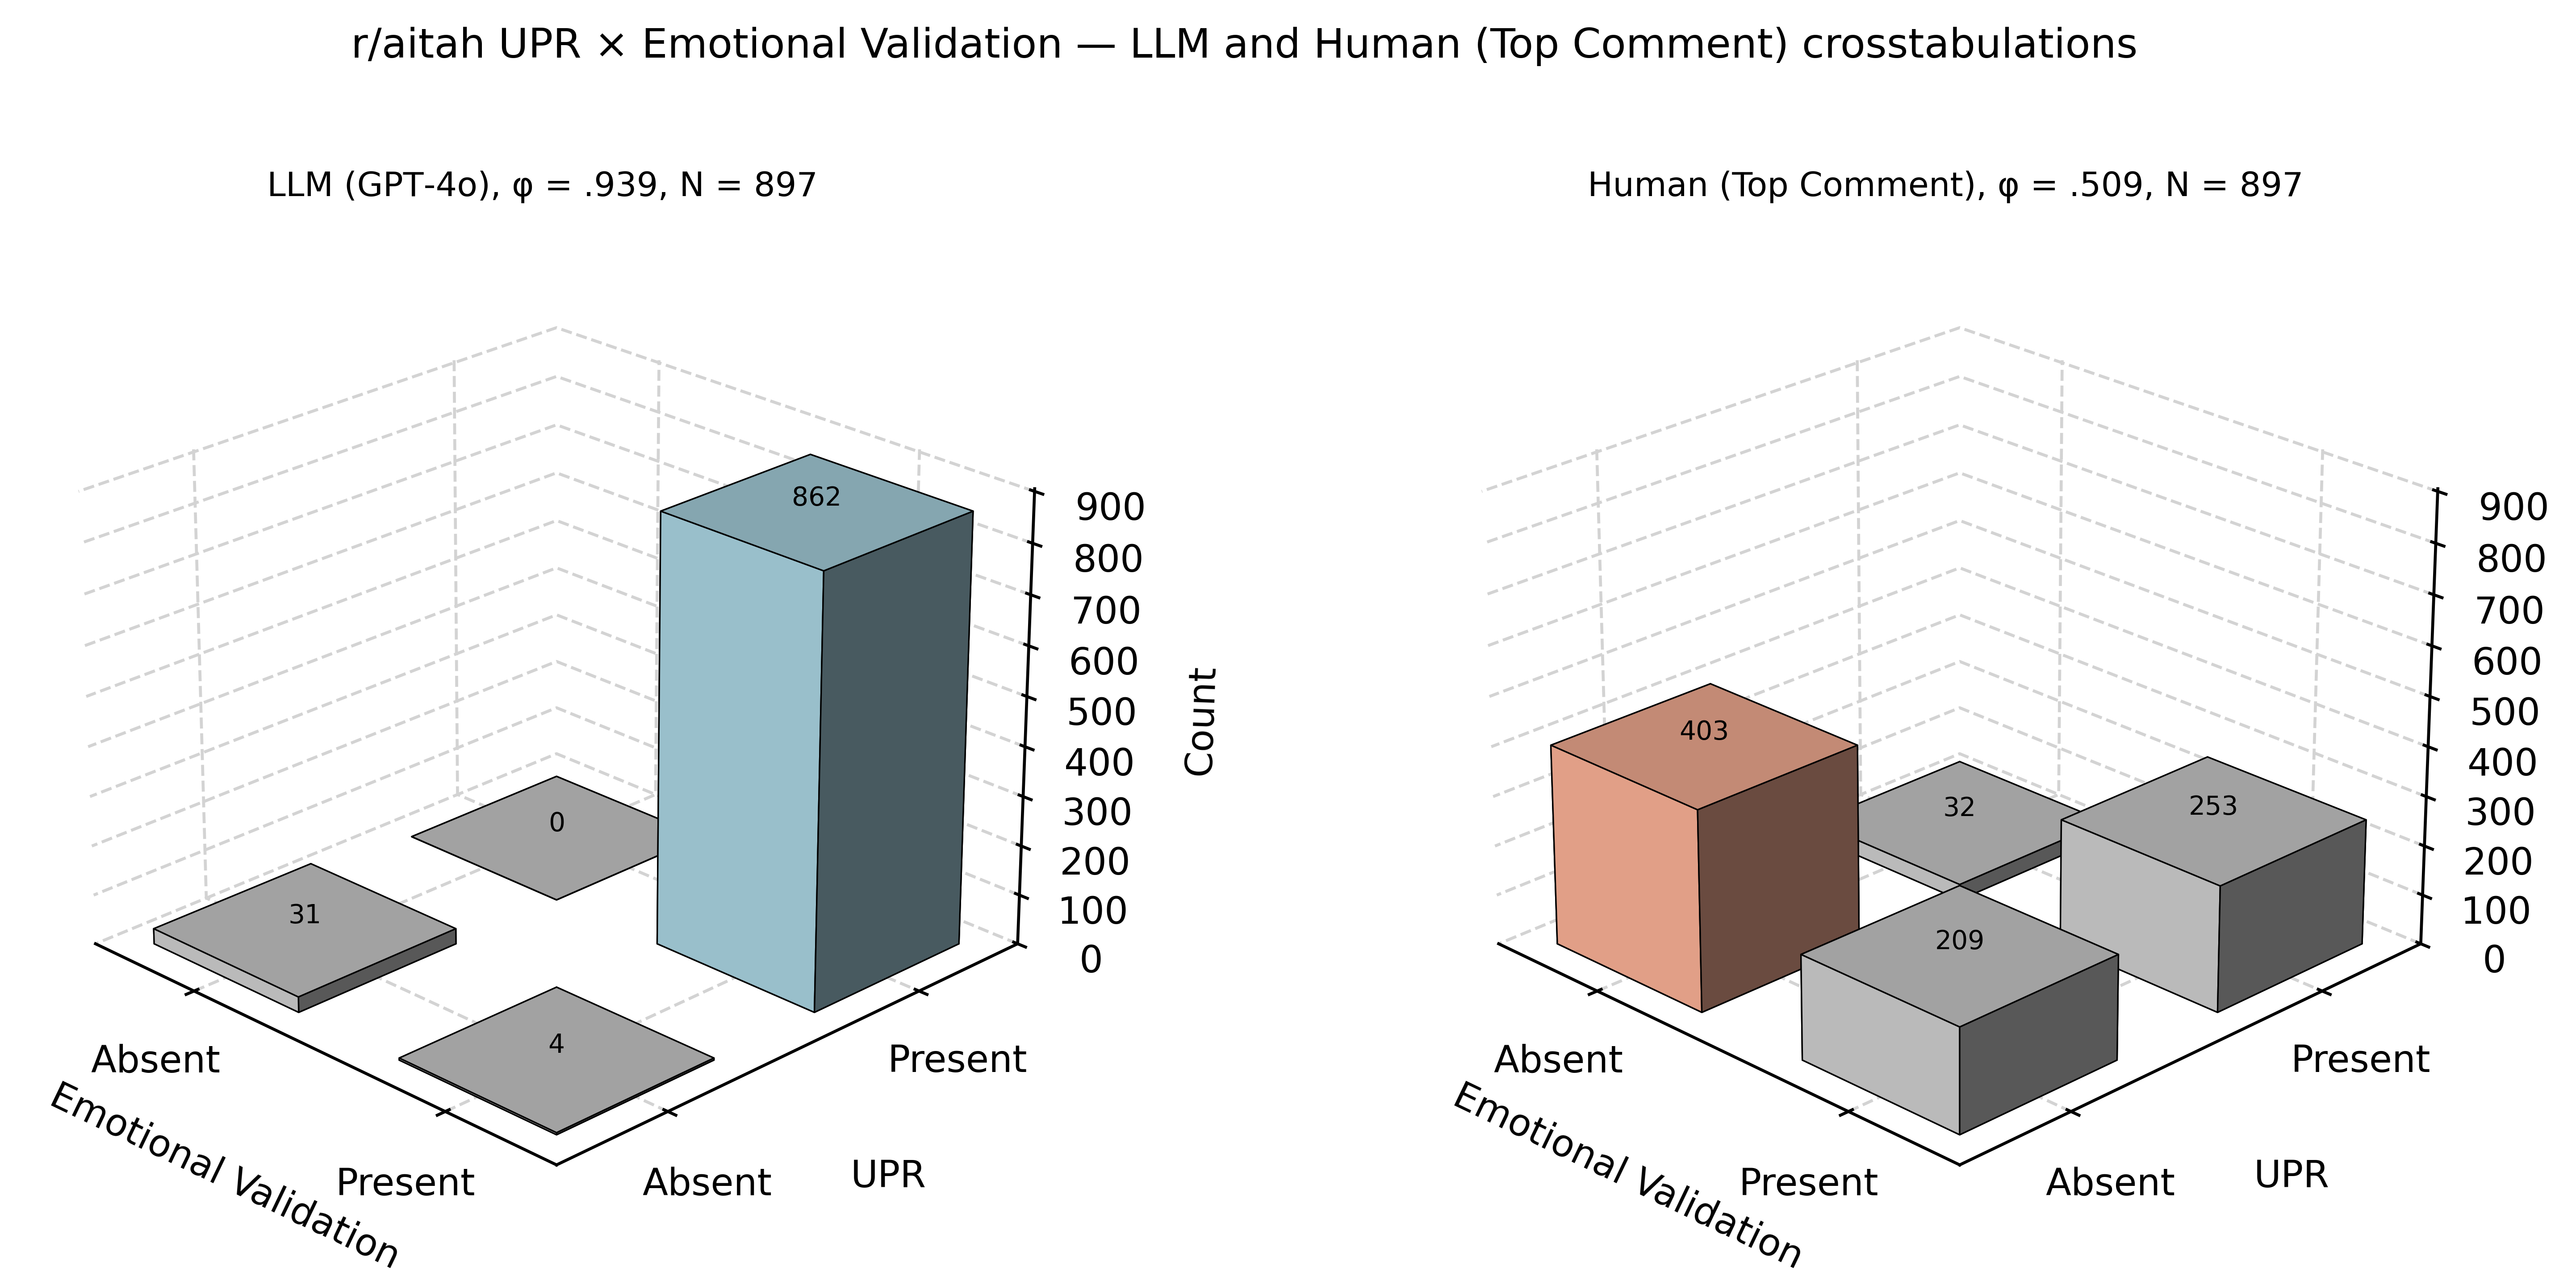
\includegraphics[width=0.9\linewidth]{Diagrams/crosstab1-upr.png}
  \caption{Cross-tabulation of Genuineness and Indirect language for the r/aitah dataset. Notice the contrasts in the presence and absence of traits between LLM-generated and human-authored responses.}
  \label{fig:crosstab1}
\end{figure}

% Insert the figure from Diagrams/crosstab1-upr.png here.
\begin{figure}[ht]
  \centering
  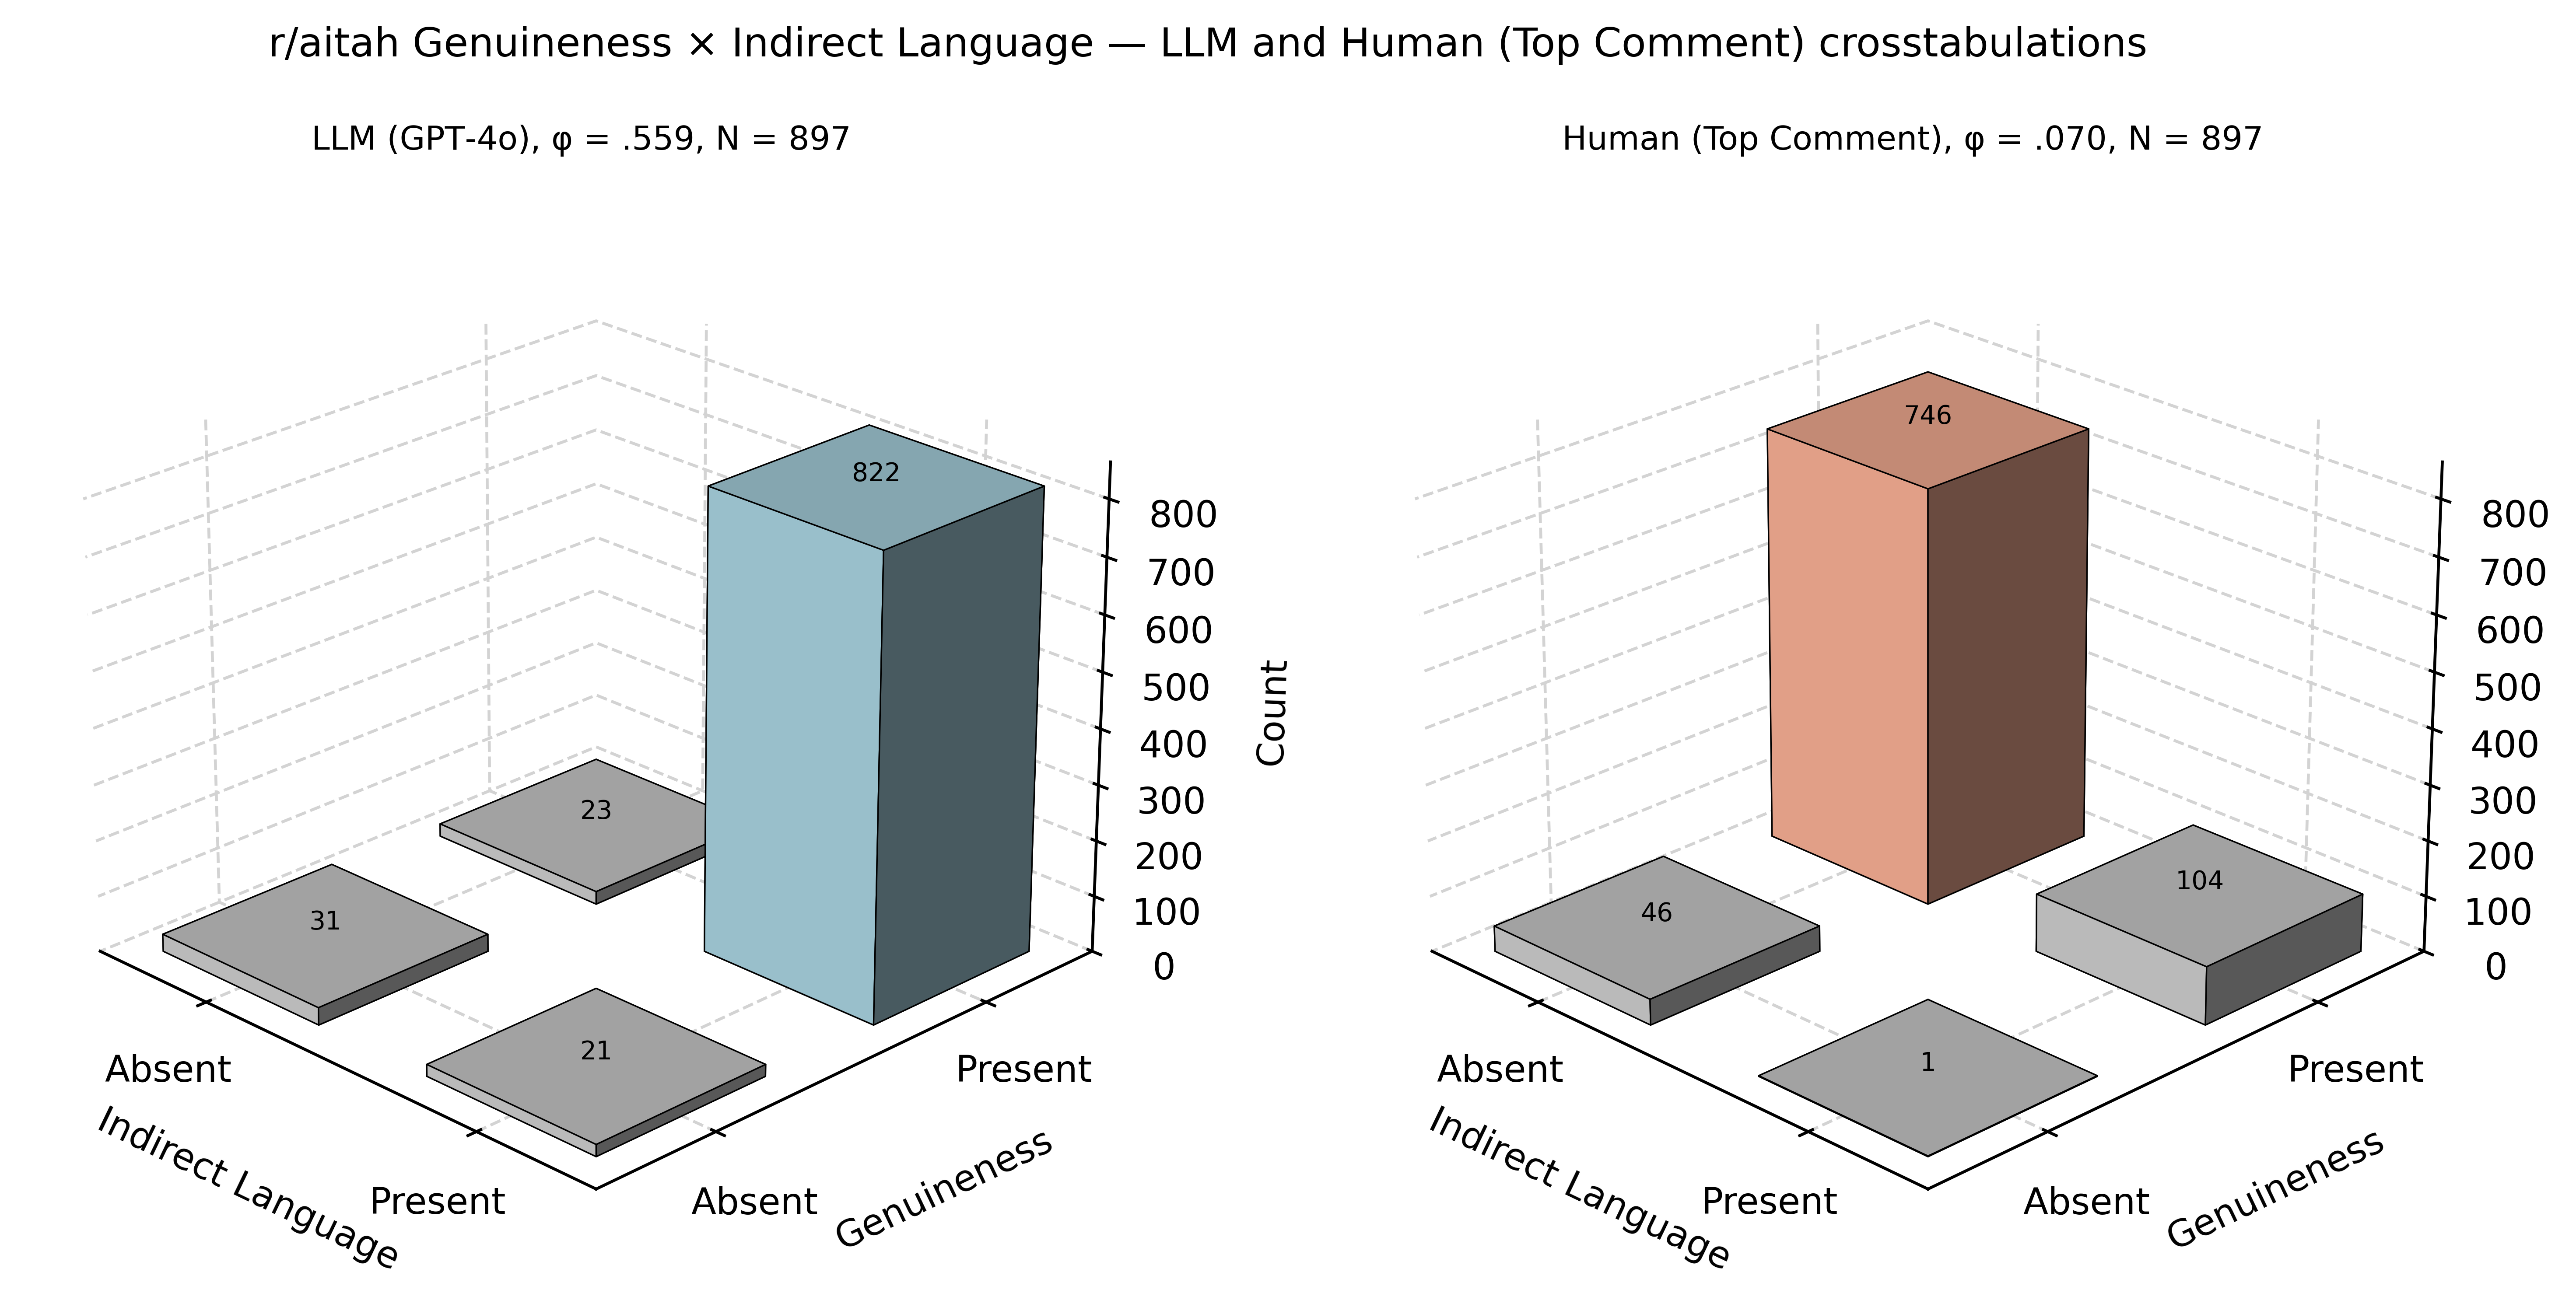
\includegraphics[width=0.9\linewidth]{Diagrams/crosstab2.png}
  \caption{Cross-tabulation of UPR and Emotional Validation for r/aitah dataset. The figure illustrates the stark contrasts in traits of LLM-generated and human-authored responses.}
  \label{fig:crosstab2}
\end{figure}

\smallskip For \textit{r/anxiety} (Table~\ref{tab:pc1.1}), the associations between UPR and Emotional Validation is moderate, with stronger effects in OP-preferred comments ($\phi = 0.369$) compared to top comments ($\phi = 0.243$). This contrasts with LLM responses in Table 2, where the strength of associations for the same measure exceeded $\phi = 0.908$ for every model considered. Similarly, trends can be seen for the \textit{r/aitah} dataset. Taken together, these results show that while human responses demonstrate overlap between empathic and sycophantic traits, the strength of association is lower relative to LLM outputs.

\smallskip Another noteworthy pattern emerges when comparing top comments with OP-preferred comments in the human authored responses. Although the sample size of responses is smaller for OP-preferred comments, owing to the fact that OPs only engaged beyond the post body in 70-75\% of the cases, the magnitude of phi is scaled by sample size and thus comparisons remain valid. 

\smallskip Across both subreddits, associations are stronger in OP-preferred comments. For example, in \textit{r/anxiety} UPR $\times$ Emotional Validation increases from $\phi = 0.243$ in top comments to $\phi = 0.369$ in OP-preferred comments. Similarly, in \textit{r/aitah}, UPR $\times$ Emotional Validation rises from $\phi = 0.509$ in top comments to $\phi = 0.544$ in OP-preferred comments. 

\smallskip \textbf{This suggests that the comments selected by original posters for engagement are more likely to exhibit overlapping the empathic and sycophantic behavioral traits than those receiving the highest community-driven endorsement through upvotes.}

\bigskip Overall, the evaluation of reddit comment responses confirms that associations between empathy- and sycophancy-related traits are present in human-authored responses too, however they occur at lower strengths than in LLM responses. The differentiation in phi between top upvoted comment and OP-preferred comments adds an additional layer of analytical insight that is directly observed from the contingency tables of annotated responses as shown in Figure~\ref{fig:crosstab1} and Figure~\ref{fig:crosstab2}.

\subsubsection{A note on human preferences in social engagement}

Across both \textit{r/anxiety} and \textit{r/aitah}, OP-preferred comments (i.e., those the OP engaged with) show higher $\phi$ associations for UPR $\times$ Emotional Validation than top comments. This suggests that OPs were more likely to interact with responses coded as ``empathic'' or ``sycophantic.'' It is worth noting, however, that OP-preferred sets are smaller ($N = 716$ vs.\ $N = 897$ for top comments in \textit{r/aitah} and $N = 752$ vs.\ $N = 935$ for top comments in \textit{r/anxiety}).

While these patterns are consistent with Cheng et al.'s observation that preference datasets underlie social ``sycophancy,'' the present analysis measures associations between annotated traits, whereas Cheng et al.\ examine dataset-level reinforcement learning preferences to determine the root cause of sycophancy\cite{cheng-etal-sycophancy}. The similarity in these findings is therefore suggestive of a shared underlying trend in preference in responses to personal questions, but it may not be deterministically conclusive. A deeper investigation of this potential connection between individual engagement patterns and large-scale reinforcement learning preference datasets lies beyond the scope of the project.

\section{Social Verdicts in r/aitah}
% Add a table here.

Since the verdict in the top comment from r/aitah can be used as a proxy for the ground truth social judgment of the situation presented by the user, the results showcase accuracy and precision scores comparing LLM judgments to human judgments. For the purposes of this project, the social verdicts were simplified into four categories: \texttt{YTA} (You are the asshole), \texttt{NTA} (Not the asshole), \texttt{REST} (Everyone sucks here or No assholes here), and \texttt{NO VERDICT} (no clear judgment).

\subsection{Generations with CoT}

\subsubsection{Shift in LLM "judgments" with CoT}\label{sec:posterchild2.2}

CoT with dialog insertion was evaluated as a control mechanism, with results varying across models. For Claude, accuracy declined from 0.45 to 0.37 and macro-average F1 from 0.41 to 0.30 with CoT insertion (Table~\ref{tab:claude_cot_comparison}). At the class level, recall for \texttt{NO VERDICT} rose from 0.12 to 0.76, while recall for \texttt{YTA} fell from 0.48 to 0.08. These results show that CoT dialog insertion redistributed performance across classes rather than producing uniform changes. Full model performances are provided in the appendix.


\begin{table}[ht]
\centering
\renewcommand{\arraystretch}{1.2}
\resizebox{\textwidth}{!}{%
\begin{tabular}{lcccc|cccc}
\toprule
\multirow{2}{*}{\textbf{Social Verdict}} 
& \multicolumn{4}{c|}{\textbf{With CoT dialog insertion}} 
& \multicolumn{4}{c}{\textbf{Without CoT dialog insertion}} \\
\cmidrule(lr){2-5} \cmidrule(lr){6-9}
 & Precision & Recall & F1-score & Support 
 & Precision & Recall & F1-score & Support \\
\midrule
NO VERDICT & 0.30 & 0.76 & 0.43 & 50 & 0.60 & 0.12 & 0.21 & 50 \\
NTA         & 0.48 & 0.62 & 0.55 & 50 & 0.38 & 0.96 & 0.55 & 50 \\
REST        & 0.50 & 0.04 & 0.07 & 50 & 0.32 & 0.23 & 0.27 & 50 \\
YTA         & 0.67 & 0.08 & 0.14 & 50 & 0.92 & 0.48 & 0.63 & 50 \\
\midrule
\textbf{Accuracy} & \multicolumn{4}{c|}{0.37 (200 comparisons)} & \multicolumn{4}{c}{0.45 (200 comparisons)} \\
\textbf{Macro avg} & 0.49 & 0.38 & 0.30 & -- & 0.55 & 0.45 & 0.41 & -- \\
\textbf{Weighted avg} & 0.49 & 0.37 & 0.29 & -- & 0.55 & 0.45 & 0.41 & -- \\
\bottomrule
\end{tabular}}
\caption{Claude performance on social judgments with and without CoT dialog insertion.}
\label{tab:claude_cot_comparison}
\end{table}

% Insert barchart 
\begin{figure}[ht]
    \centering
    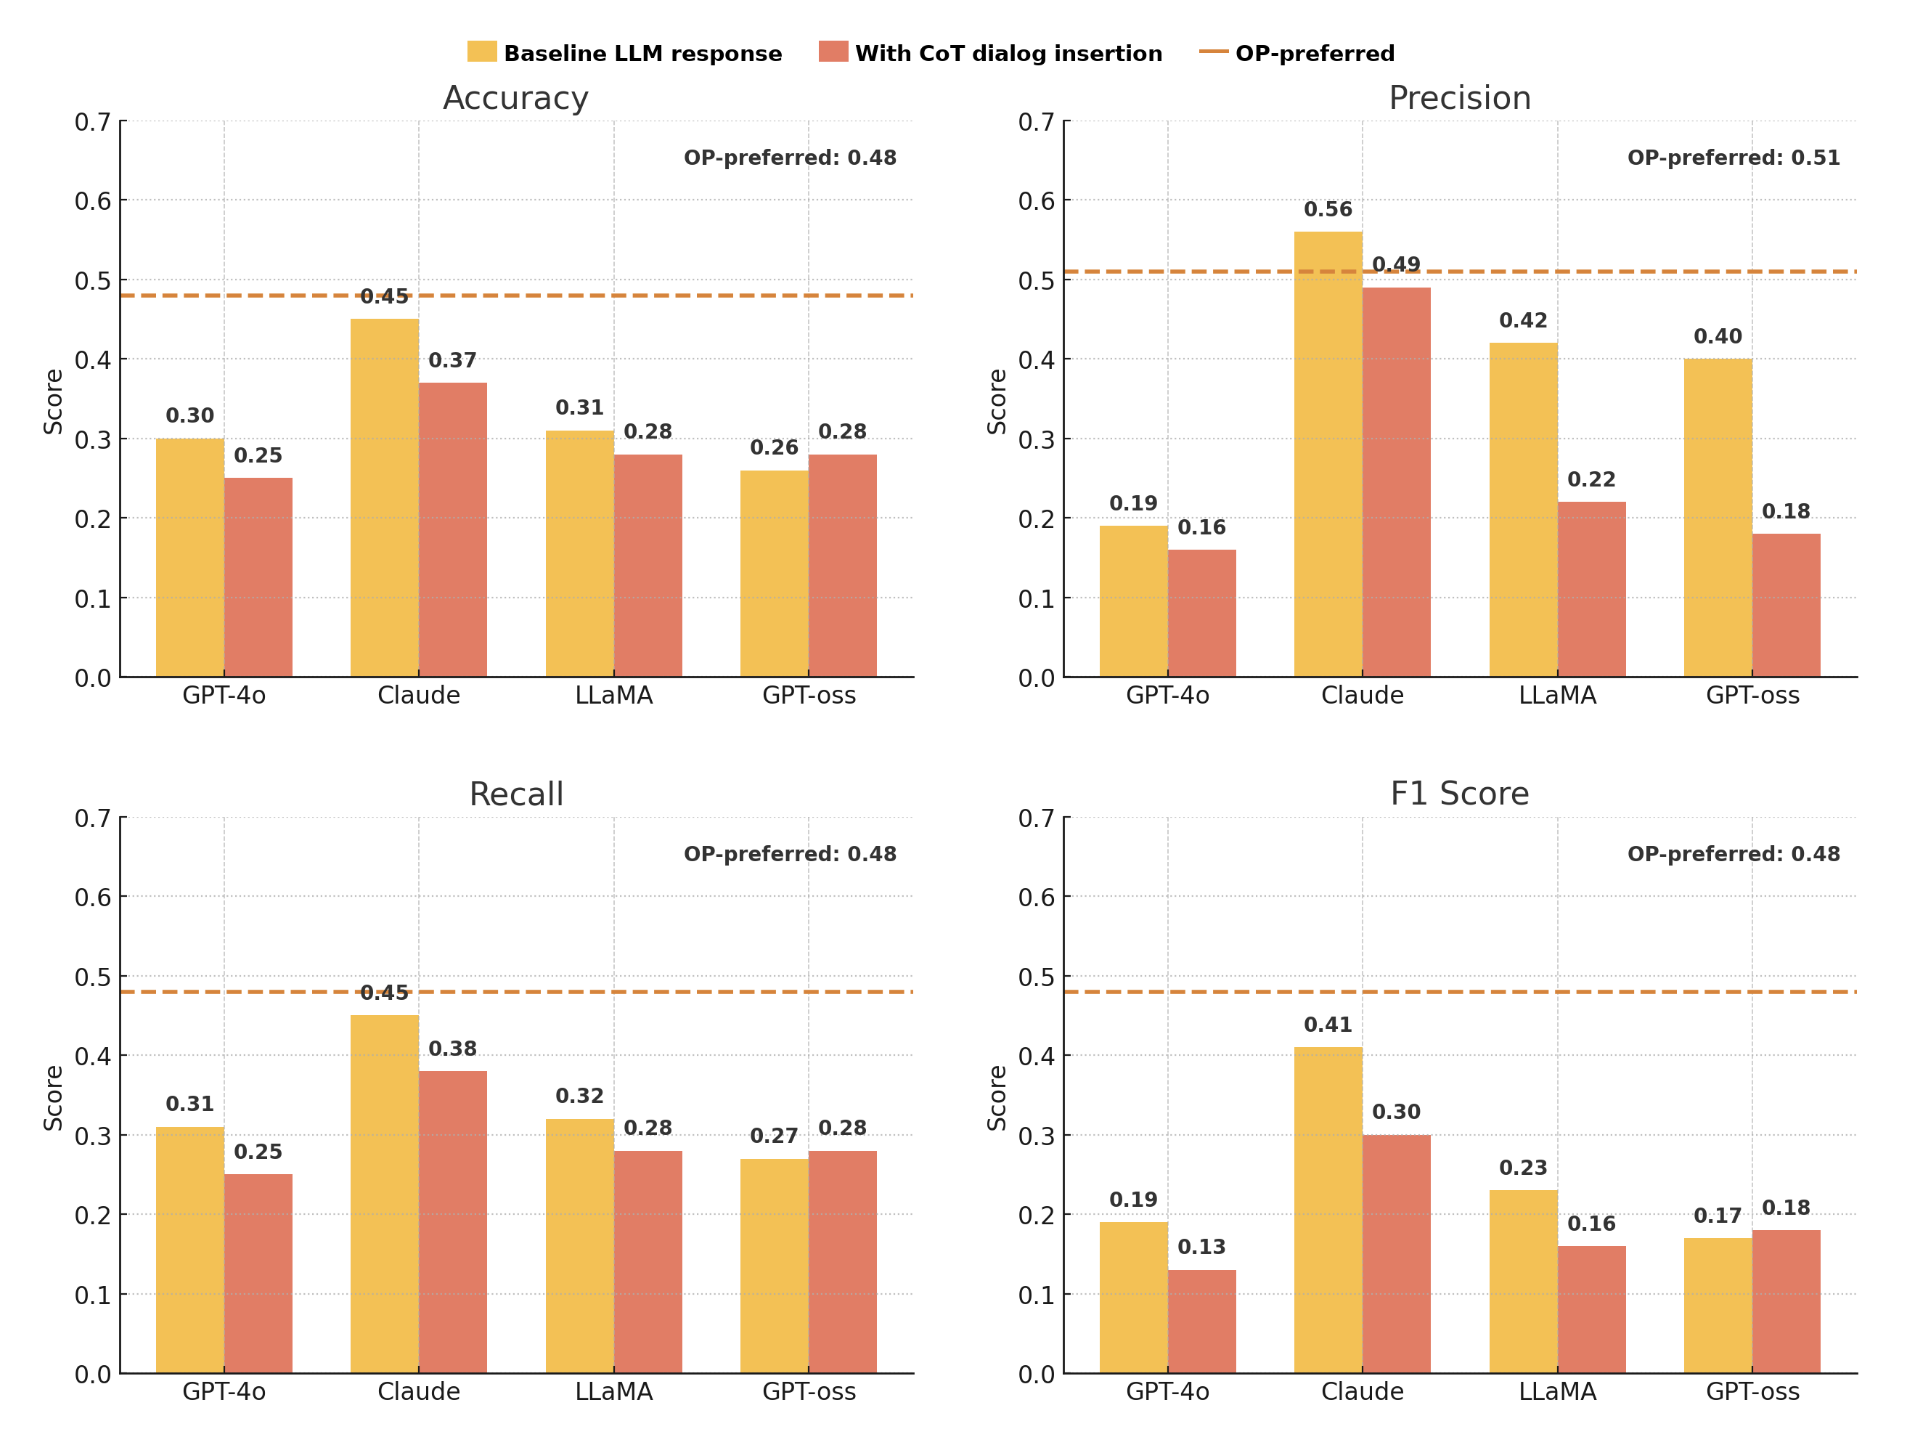
\includegraphics[width=0.9\linewidth]{Diagrams/verdicts_2.png}
    \label{fig:social_verdicts}
    \caption{\textit{r/aitah}---Overall performance scores (Accuracy, Precision, Recall, and F1 Score) for OP-preferred responses and model outputs (GPT-4o, Claude, LLaMA, GPT-oss), comparing model baseline response with CoT dialog insertion. Values represent aggregate scores across the four classes, not per-class results.}
\end{figure}

Across models, CoT dialog insertion did not consistently raise or lower overall metrics such as accuracy or F1. Instead, it shifted the balance of social judgments, with some classes gaining in recall or precision and others showing losses. While the results depicted may provide a useful starting point for investigation in this area, further study is necessary to determine how CoT dialog insertion affects model outputs in the context of personal queries.


Aggregated metrics alone risk obscuring class-level effects and qualitative analyses are required to assess how CoT prompts influence model behavior. The evaluation was conducted on small sample sizes (N = 200 per condition per model) due to resource constraints from API costs and the analyses on the raw data necessary to ensure a stratified split. While trends are visible, they should be interpreted cautiously. The implications of limited sample size for generalizability are addressed in the limitations section \ref{sec:limitations}.

% Can add a note in the analyses saying that these results match the findings of Cheng et al. on sycophancy where no mitigation stretegy was found to be consistently effective across models.

% TODO: Speak to the annotations missing out on sarcasm and nuanced communication. Showcase examples in the report.
